\documentclass[12pt]{article}


\usepackage[
    a4paper, 
    margin=2.5cm]{geometry}
\usepackage[utf8]{inputenc}         % UTF8 enkodiranje
\usepackage[slovene]{babel}          % Slovenščina
\usepackage[
    pdfusetitle, 
    hidelinks, 
    unicode]{hyperref}              % Nastavi atribute PDF-ja, ne označuj povezav
\usepackage{microtype}              % Izboljšave za tipografijsko perfekcijo :)
\usepackage{enumitem}               % Seznami za člene
\usepackage{graphicx}               % Vključitev slik
\usepackage{dirtytalk}              % Citat
\usepackage{listings}               % Kodni blok
\usepackage{fancyvrb}
\usepackage[font=]{caption}         % Required for specifying captions
\usepackage[normalem]{ulem}         % Krašanje enot v enačbi
\usepackage{times}                  % Times New Roman pisava
\usepackage{tikz} 
\usetikzlibrary{patterns}
\usetikzlibrary{arrows}
\usepackage[european]{circuitikz}   % Električna vezja
\usepackage{datetime}               % Datum
% \usepackage[slovenian]{csquotes}
\usepackage{braket}
\usepackage{amsmath} % matematika ki izgleda lepo
\usepackage{amsfonts} % množice
\usepackage[style=ieee, maxbibnames=3, minbibnames=1, 
maxcitenames=1, mincitenames=1, sorting=nyt]{biblatex}   % Navajanje virov
\bibliography{viri}

\urlstyle{rm}

\setlength{\parindent}{0em}
\setlength{\parskip}{1ex}

\setcounter{secnumdepth}{5}
\setcounter{tocdepth}{4}

\renewcommand{\thesection}{\arabic{section}}
\renewcommand{\thesubsection}{\thesection.\arabic{subsection}}
\renewcommand{\thesubsubsection}{\thesubsection.\arabic{subsubsection}}
\renewcommand{\theparagraph}{\thesubsubsection.\arabic{paragraph}}
\renewcommand{\thesubparagraph}{\theparagraph.\arabic{subparagraph}}

\renewcommand{\labelnamepunct}{\addcomma\space}
\DeclareFieldFormat[article]{title}{#1}
\DeclareFieldFormat[online]{title}{\mkbibemph{#1}}

\DefineBibliographyStrings{slovene}{
    andothers = {et. al\adddot},
    urlseen = {dostopano:}
}
    % Adapted from the 'patterns' library: enlarged the distance between the lines from 4pt to 10pt
\pgfdeclarepatternformonly{north east lines wide}{\pgfqpoint{-1pt}{-1pt}}{\pgfqpoint{10pt}{10pt}}{\pgfqpoint{9pt}{9pt}}%
{
    \pgfsetlinewidth{0.4pt}
    \pgfpathmoveto{\pgfqpoint{0pt}{0pt}}
    \pgfpathlineto{\pgfqpoint{9.1pt}{9.1pt}}
    \pgfusepath{stroke}
}


\tikzset{%
    body/.style={inner sep=0pt,outer sep=0pt,shape=rectangle,draw,thick,pattern=north east lines wide},
    dimen/.style={<->,>=latex,thin,every rectangle node/.style={fill=white,midway,font=\sffamily}},
    symmetry/.style={dashed,thin},
}
    
\newdateformat{MMYYYYdate}{\monthname[\THEMONTH] \THEYEAR}

\title{Poročila maturitetnih vaj pri predmetu fizika}
\author{Jaka Kovač, G 4. b}

\begin{document}
\pagenumbering{arabic}

\begin{center}
    \thispagestyle{empty}
    \includegraphics[scale=1]{slike/logotip_vegova_leze_brezokvirja.png}
    \\
    \textbf{Vegova ulica 4, 1000 Ljubljana}

    \vspace{\fill} 
    Poročila vaj pri predmetu fizika

    \Huge{\textbf{Poročila maturitetnih vaj}}

    \normalsize
    \vspace{\fill}

    Mentor: Tomo Omahna, prof. \hfill Avtor: Jaka Kovač, G 4. b\\
    \null
    Ljubljana, oktober 2023 – \MMYYYYdate\today %zamenjaj <mesec in leto> z mesecem in letom začetka
\end{center}
\newpage
\thispagestyle{empty}
\null
\newpage

\section*{Povzetek}
V tem delu bom predstavil kako sem izvedel maturitene vaje, njihove rezultate. Ob vsaki vaji
sem preverjal veljavnost meritev s teoretično izračunaimi vrednostmi.
\\ %prazna vrstica
\textbf{Ključe besede:} poročila maturitetnih vaj - fizika, fizika za srednjo šolo

\vfill
\section*{Abstract}
\foreignlanguage{english}{This paper describes how to use \LaTeX{} to write a paper.
\\ %prazna vrstica
\textbf{Keywords:} \LaTeX{}, paper, \LaTeX{} template}
\vfill

% KAZALO 
\newpage
\thispagestyle{empty} % ne številčimo strani
\tableofcontents % kazalo

\begingroup     % kazalo slik
\makeatletter
\section*{Slike}
\@starttoc{lof}
\let\clearpage\relax
\makeatother
\endgroup


\newpage

\section*{O zapisu meritev}
Prikazane številčne vrednosti so zaokrožene na 3 od 0 različna decimalna mesta (znanstven zapis).
V izračunih se uporablja dejanska vrednost. Kjer ni drugače navedeno je vrednost podana na
$\pm 0.5$ enot na zadnjem prikazanem mestu. Primer: $s = 10.0 \text{ m} = 10.0 \text{ m} \pm 0.05 \text{ m}$

\section{Lastno nihanje vzmetnega nihala}
    \subsection*{Opis vaje in teoritična podlaga}
    \subsection*{Uporabljeni pripomočki}
    \subsection*{Grafi, ipd.}
    \subsection*{Analiza rezultatov}

\newpage
\section{Prosti pad}
    \subsection*{Opis vaje in teoritična podlaga}
    \subsection*{Uporabljeni pripomočki}
    \subsection*{Grafi, ipd.}
    \subsection*{Analiza rezultatov}

\newpage
\section{Odbojnost}
    \subsection*{Opis vaje in teoritična podlaga}
    \subsection*{Uporabljeni pripomočki}
    \subsection*{Grafi, ipd.}
    \subsection*{Analiza rezultatov}

\newpage
\section{Boylov zakon}
    \subsection*{Opis vaje in teoritična podlaga}
    \subsection*{Uporabljeni pripomočki}
    \subsection*{Grafi, ipd.}
    \subsection*{Analiza rezultatov}

\newpage
\section{Atwoodovo padalo}
    \subsection*{Opis vaje in teoritična podlaga}
    \subsection*{Uporabljeni pripomočki}
    \subsection*{Grafi, ipd.}
    \subsection*{Analiza rezultatov}

\newpage
\section{Dušeno nihanje v električnem krogu}
    \subsection*{Opis vaje in teoritična podlaga}
    Cilj vaje je izračunati koeficient dušenja $\beta$ v dušemen električnem nihajenm krogu.
    
    \subsection*{Uporabljeni pripomočki}
    \subsection*{Grafi, ipd.}
    \subsection*{Analiza rezultatov}

\newpage
\section{Gostota zemljinega električnega polja}
    \subsection*{Opis vaje in teoritična podlaga}
    \subsection*{Uporabljeni pripomočki}
    \subsection*{Grafi, ipd.}
    \subsection*{Analiza rezultatov}

\newpage
\section{Merjenje goriščne razdalje leč}
    \subsection*{Opis vaje in teoritična podlaga}
    Vaja zajema merjenje goriščne razdalje konveksne (zbiralne), konkavne (razpršilne) in 
    stavljene leče. Formula za izračun goriščne razdalje leče je $f = 2R$, kjer je $f$ 
    goriščna razdalja, $R$ pa polmer leče ali zrcala. Goriščna razdalja sestavljene leče
    (dve zaporedni leči) se izračuna z $\frac{1}{f} = \frac{1}{f_1} + \frac{1}{f_2} - \frac{d}{f_1 \cdot f_2}$
    \cite{lece}, kjer sta $f_1$ in $f_2$ goriščni razdalji sestavnih leč, $d$ pa razdalja med njima.

    \subsection*{Uporabljeni pripomočki}
    Svetilka v ohišju z režami, ŠMI z vezicami, milimeterski papir, svinčnik, geotrikotnik, 
    konveksna in konkavna leča ($R = 35 \text{ mm}$ za obe leči)
    \subsection*{Skice}
    
    %Zbiralna leča
    \begin{figure}[h!]
        \centering
        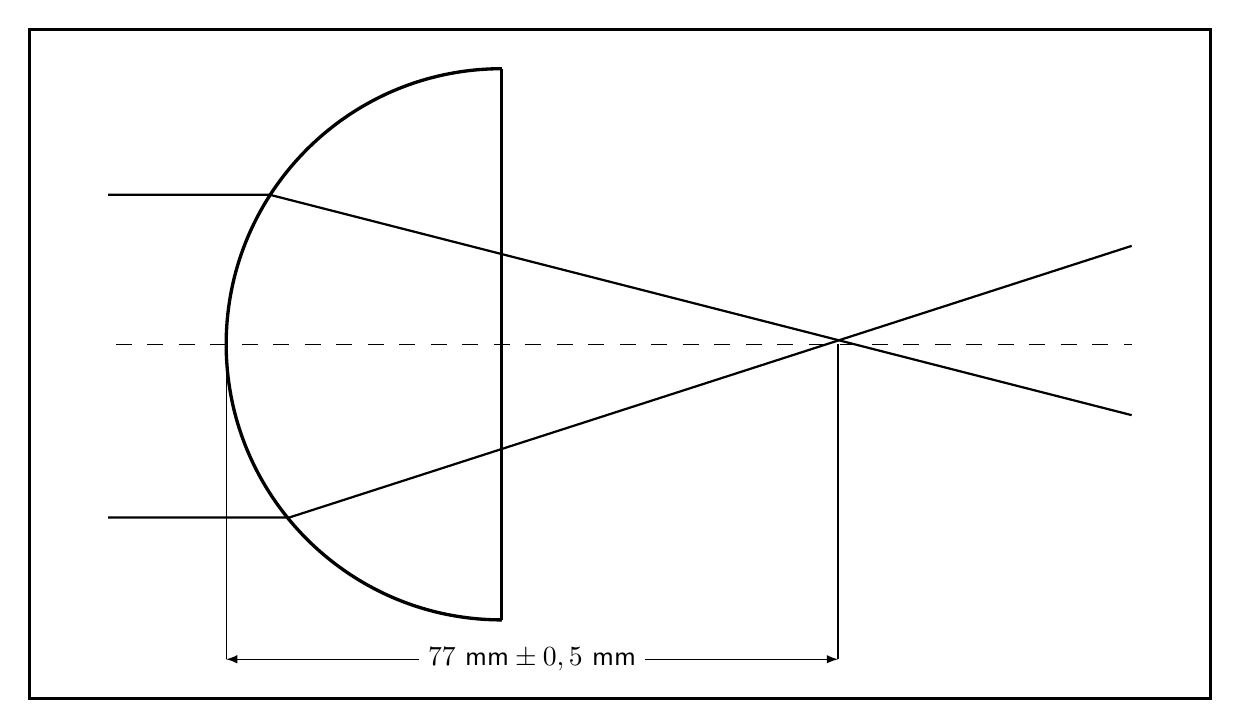
\begin{tikzpicture}
            \draw[black, very thick] (-6,-4.5) rectangle (9,4);
            \draw[dash=on 2mm off 2mm phase -1mm] (-5, 0) -- (8, 0);
                
            %leča
            \draw[very thick] (0, 3.5) arc (90:270:3.5);
            \draw[very thick] (0, 3.5) -- (0, -3.5);
            
            %žarki
            \draw[thick] (-5, 1.9) -- (-2.95, 1.9) -- (8, -0.9);
            \draw[thick] (-5, -2.2) -- (-2.7, -2.2) -- (8, 1.25);
            
            %meritev
            \draw (-3.5, 0) -- (-3.5, -4);
            \draw (4.27, 0) -- (4.27, -4);
            \draw[dimen] (-3.5, -4) -- (4.27, -4) node {$77 \text{ mm} \pm 0,5 \text{ mm}$};
        \end{tikzpicture}
        \caption{Zbiralna leča}
    \end{figure}
    
    %Razpršilna leča
    \begin{figure}[h!]
        \centering
        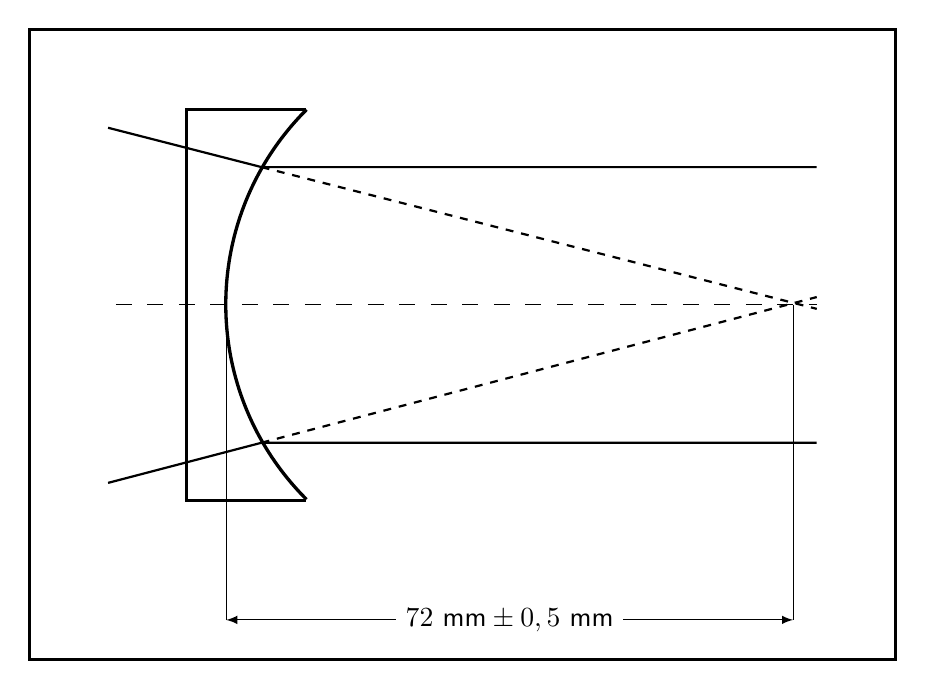
\begin{tikzpicture}
            \draw[black, very thick] (-6,-4.5) rectangle (5, 3.5);
            \draw[dash=on 2mm off 2mm phase -1mm] (-5, 0) -- (4, 0);
            
            %leča
            \draw[very thick] (-2.48, 2.48) arc (135:225:3.5);
            \draw[very thick] (-2.48, 2.48) -- (-4, 2.48) -- (-4, -2.48) -- (-2.48, -2.48);
            
            %žarki
            \draw[thick] (4, 1.75) -- (-3.05, 1.75) -- (-5, 2.25);
            \draw[thick] (4, -1.75) -- (-3.05, -1.75) -- (-5, -2.26);
            \draw[thick, dash=on 1mm off 1mm phase 0mm] (-3.05, 1.75) -- (4, -0.05);
            \draw[thick, dash=on 1mm off 1mm phase 0mm] (-3.05, -1.75) -- (4, 0.1);
            
            %meritev
            \draw (-3.5, 0) -- (-3.5, -4);
            \draw (3.7, 0) -- (3.7, -4);
            \draw[dimen] (-3.5, -4) -- (3.7, -4) node {$72 \text{ mm} \pm 0,5 \text{ mm}$};
        \end{tikzpicture}
        \caption{Razpršilna leča}
    \end{figure}
    
    %Sestavljena leča
    \begin{figure}[h!]
        \makebox[\textwidth][c]{
            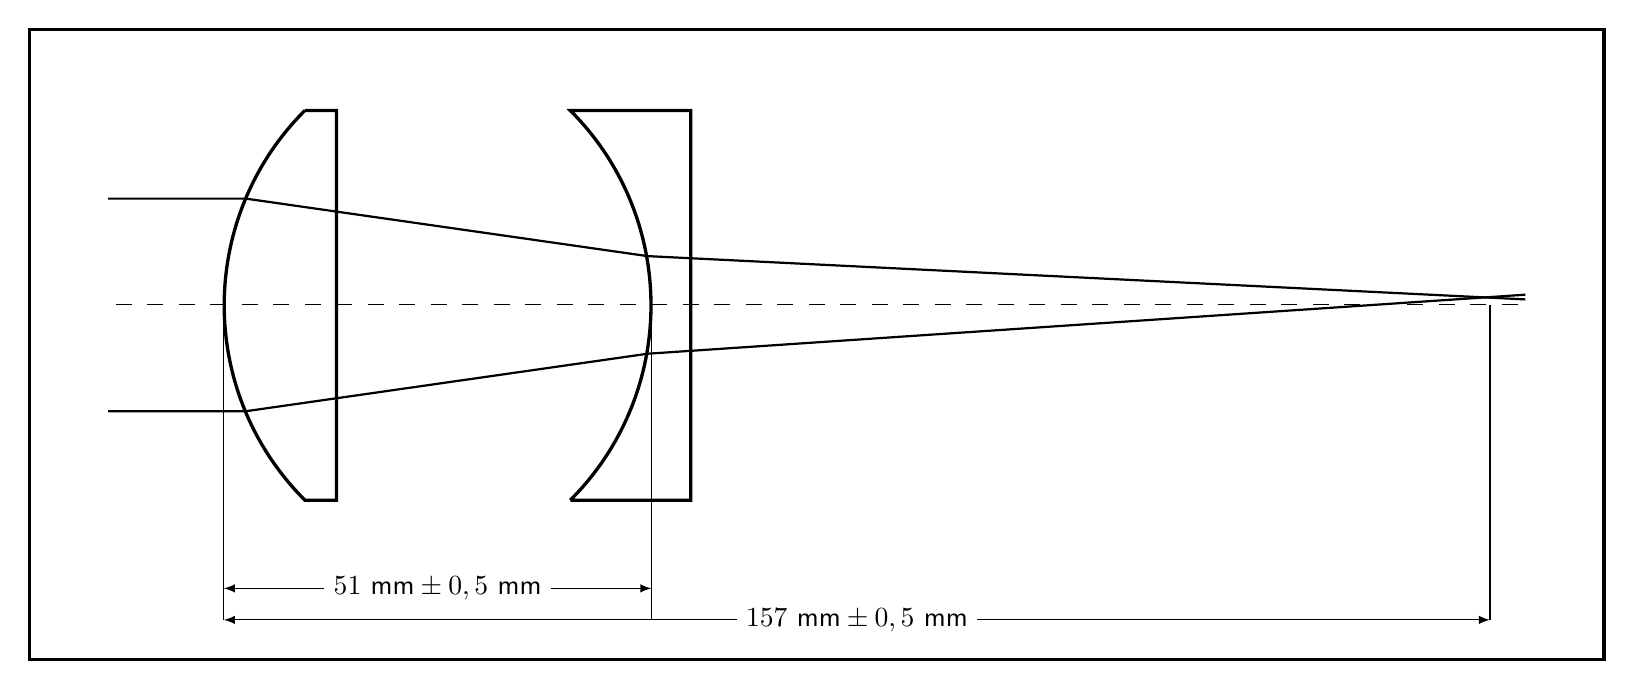
\begin{tikzpicture}
                \draw[black, very thick] (-10,-4.5) rectangle (10, 3.5);
                \draw[dash=on 2mm off 2mm phase -1mm] (-9, 0) -- (9, 0);
                
                %zibralna leča
                \draw[very thick] (-6.5, 2.47) arc (135:225:3.5) -- (-6.1, -2.48) -- (-6.1, 2.47) -- (-6.5, 2.47);
                
                %razpršilna leča
                \draw[very thick] (-3.13, -2.48) arc (-45:45:3.5) -- (-1.6, 2.47) -- (-1.6, -2.48) -- (-3.13, -2.48);
                
                %žarki
                \draw[thick] (-9, 1.35) -- (-7.25, 1.35) -- (-2.15, 0.62) -- (9, 0.07);
                \draw[thick] (-9, -1.35) -- (-7.25, -1.35) -- (-2.15, -0.62) -- (9, 0.13);
                
                %meritve
                \draw (-7.53, 0) -- (-7.53, -4);
                \draw (8.55, 0) -- (8.55, -4);
                \draw[dimen] (-7.53, -4) -- (8.55, -4) node {$157 \text{ mm} \pm 0,5 \text{ mm}$};
                \draw (-2.1, 0) -- (-2.1, -4);
                \draw[dimen] (-7.53, -3.6) -- (-2.1, -3.6) node {$51 \text{ mm} \pm 0,5 \text{ mm}$};
            \end{tikzpicture}
            }
        \caption{Sestavljena leča}
    \end{figure}
    \newpage
    \subsection*{Analiza rezultatov}
    Izmerjena goriščna razdalja konveksne leče je $f = 77 \text{ mm} \pm 0,5 \text{ mm}$,
    izračunana razdalja pa je 
    \begin{equation}
        f = 2R = 2 \cdot 35 \text{ mm} = 70 \text{ mm}
    \end{equation}.\\
    Za konkavno lečo pa sem izmeril goriščno razdaljo $f = 72 \text{ mm} \pm 0,5 \text{ mm}$, 
    izračunana goriščna razdalja je 
    \begin{equation}
        f = -2R = -2 \cdot 35 \text{ mm} = -70 \text{ mm}
    \end{equation}.\\
    Pri sestavljeni lečo sem izmeril goriščno razdaljo $f = 157 \text{ mm} \pm 0,5 \text{ mm}$,
    izračunal pa sem
    \begin{equation}
        \begin{split}
            \frac{1}{f} &= \frac{1}{f_1} + \frac{1}{f_2} - \frac{d}{f_1 \cdot f_2} \\
            f &= (\frac{1}{-70 \text{ mm}} + \frac{1}{70 \text{ mm}} - \frac{51 \text{ mm}}{-70 \text{ mm} \cdot 70 \text{ mm}})^{-1}\\
            f &= 102 \text{ mm}
        \end{split}
    \end{equation}
    če za izračun uporabimo izmerjene vrednosti dobimo, da je goriščna razdalja $f = 120 \text{ mm}$.
    Kljub vsemu osnovne formule za izračun goriščne razdalje sestavljene leče sam ne morem
    potrditi.


\newpage
\section{Plinski emisijski spektri}
    \subsection*{Opis vaje in teoritična podlaga}
    \subsection*{Uporabljeni pripomočki}
    \subsection*{Grafi, ipd.}
    \subsection*{Analiza rezultatov}



\newpage
\begingroup
\makeatletter
    \section{Viri in literatura}
    \nocite{*}
    \printbibliography[heading=none]
\makeatother
\endgroup
\newpage

\begin{samepage}
    \thispagestyle{empty}
    \section*{Izjava o avtorstvu}
    Izjavljam, da je seminarska naloga v celoti moje avtorsko delo, ki sem ga 
    izdelal samostojno s pomočjo navedene literature in pod vodstvom mentorja.

    \vfill
    
    \today \hfill Jaka Kovač
    
    \vspace{3 cm}
\end{samepage}

\end{document}
